% !TEX root = ../main.tex


% = = = = = = = = = = = = = = = = = = = = = = = = = = = = = 
% = = = Intro 
% = = = = = = = = = = = = = = = = = = = = = = = = = = = = = 

\section{Introduction}

Consider the traditional multi-party computational setting with a twist: Alice and Bob each have some data, they would like to know the output from running an agreed-upon function on their data, each does not want the other (or anyone else) to learn their data, and they want to simply submit their data (\eg encrypted) to a trustworthy system and come back later for the result. They are willing to pay for this service and understand that, in the worst case of massive collusion between the operators of this service (called trustees), their inputs may be exposed but the result will always be correct.

We assume the reader is familiar with blockchain technology, Ethereum, and smart contracts or decentralized apps (DApps). Can these technologies help? In theory? In practice? We seek to answer this question through direct experimentation. The abstract above builds the argument for why blockchain can help: (1) it provides an integral point of coordination where trustees can post and track progress on the evaluation; (2) it provides an in-band solution for paying the trustees (in either a cryptocurrency like ETH or in a stablecoin pegged to the value of governmental currency like the USD) in a way that is contingent on their performance; and (3) it can serve as the public verifier and can reject any protocol proof that is not correct. When Alice and Bob retrieve the result (whether in plaintext or individually encrypted under their keys), they know it must be correct, otherwise it would not be there waiting for them.

Our experiments show that while in theory the idea is sound and we are able to successfully perform a secure function evaluation of a single logic gate (NAND gate) on Ethereum, the costs today are too prohibitive for it to be considered practical. We then turn to so-called layer-2 solutions and show that Arbitrum (an optimistic roll-up that is based on the same trustee model we are already using~\cite{KGCWF18} can make Absentia substantially more practical (with room for further improvement).
 
% = = = = = = = = = = = = = = = = = = = = = = = = = = = = = 
% = = = Design Decisions 
% = = = = = = = = = = = = = = = = = = = = = = = = = = = = = 
 
\subsection{Key design decisions}

Note that we use the term secure function evaluation (SFE) to describe the stateless, one-shot evaluation that Absentia provides; and reserve the term multiparty computation (MPC) ~\textcolor{red}{for a more setting} where stateful computations might be performed over time.

\paragraph{Design decision: Trustee model.} In keeping with our priority for a submit-and-go protocol, someone has to perform the actual evaluation of the function on the inputs. We call these entities \emph{trustees}. We assume the number of trustees ($n$) can be chosen independently of the number of inputs. ~\textcolor{red}{In Absentia, we simply our implementation} to only support robustness in the case that all trustees ($n$-out-of-$n$) participate, however this could be modified to allow the protocol to proceed if only a threshold ($t$ out of $n$ for some $t<n/2$) of trustees participate (this, however, also reduces the number of trustees that need to collude to break the privacy, and potentially correctness, of the protocol).  

The remaining question is how can Alice and Bob find trustees they assume will not collude? We have several suggestions: (1) it could be based on personal connections; (2) perhaps commercial entities would emerge with either pre-established reputations or earn their reputation over time (similar to oracle providers) and through legally enforceable terms of service; or (3) trustees could be picked at random from a large set of trustees. While (3) may not sound convincing, it is essentially same threat model as the anonymous web-browsing tool Tor which is trusted by vulnerable users (perhaps Tor also uses flavours of (1) via its EntryGuard program). 

\paragraph{Design decision: Ethereum.} While we are not the first to explore multi-party computation and its relationship to blockchain (see Section~\ref{sec:lit}), we believe we are the first to implement an MPC protocol on a public, commonly used blockchain; namely, Ethereum. The first research question ~\textcolor{red}{we is whether} MPC is even feasible on Ethereum, given the heavy cryptography it uses. Our paper establishes a benchmark that we hope to see improved through future research. Ethereum itself has scheduled scalability plans including Ethereum 2.0 (more transactions per second), and a lot of community resources are also being spent examining and implementing \emph{layer 2} solutions that move blockchain functionality off of the main chain without sacrificing many of its security benefits. Technologies include \emph{state channels}, \emph{sidechains}, and \emph{roll-ups}~\cite{GMR+20}. To experiment with these technologies, we also deploy and benchmark critical components of Absentia on Arbitrum~\cite{KGCWF18}, a recently proposed system for optimistic roll-ups (describe more in Section~\ref{sec:arb}). We now turn to another avenue for improvement, using state-of-the-art MPC protocols.

\paragraph{Design decision: Mix and match.} Starting with Yao in 1982~\cite{Yao82}, the question of how to securely evaluate a general function, when inputs are held by multiple people, has generated a rich body of literature in cryptography. In choosing an SFE/MPC protocol for the basis of Absentia, we looked for one with the following properties:

\begin{enumerate}
\item \textbf{Trustee model.} As justified above, we seek an MPC/SFE protocol that lets the input holders (\eg Alice and Bob) offload their inputs to a set of non-colluding trustees for evaluation. 
\item \textbf{Publicly verifiable} (aka publicly auditable or universally verifiable). Many MPC/SFE protocols are in the semi-honest (\ie honest-but-curious) model. Some are resilient to covert or malicious adversaries. We require that not only can adversarial behaviour  be detected by the participates in the protocol, but that it can be detected by anyone (\ie the public). This allows (a) Alice and Bob to offload the computational work to the trustees and still ensure the output is correct, even if they did not directly participate, and (b) Alice and Bob can go further and offload the verification itself to someone they trust---the Ethereum network in this case.
\item \textbf{Identifiable aborts.} If the protocol does not reach completion, anyone can establish which trustee aborted.
\item \textbf{Elliptic curve operations.} While Ethereum can in theory implement different types of cryptography (RSA groups, integer-based discrete logarithms groups, lattices, \etc), it has native support for its own cryptographic operations (ECDSA signatures) on the elliptic curve \texttt{secp256k1}. For ease of implementation, we prefer a SFE/MPC with the same cryptographic setting. 
\item \textbf{Circuit type.} When the function to be evaluated is represented as a circuit, the circuit could be based on logic gates (\ie NAND gates) or arithmetic operations (\eg additions and multiplications in a modular group). We are indifferent to this design parameter.
\end{enumerate}

One SPF protocol to meet our purposes is Mix and Match~\cite{JJ00} and we chose it based on our familiarity with it. We are also aware that the state-of-the-art MPC protocols are based on a different paradigm---based on \emph{Beaver triples}~\cite{beaver1997commodity}---initiated by the SPDZ protocol~\cite{damgaard2012multiparty,damgaard2013practical} with many followups (HighGear is a recent example~\cite{keller2018overdrive}). While SPDZ uses lattice-based somewhat homomorphic encryption (SME), this is during a pre-computation phase and Absentia (for now) assumes all pre-computation has been validated. SPDZ also appears amenable to a trustee model and one paper explores a publicly verifiable variant~\cite{baum2014publicly}, however since the authors do not compare themselves to Mix and Match, it would be a complete research project to determine if it is indeed faster. We note that it is not obviously categorically faster---for example, by not requiring public key operations at all: the publicly verifiable variant uses Pedersen commitments extensively.  

We are not aware of an explicit \emph{proof} that Mix and Match is publicly verifiable, however every step of the protocol is covered by a trustee issuing a non-interactive zero knowledge proof and it is later assumed to be by the authors in their auction application~\cite{JJ00}. Stated a different way, it appears that even when all trustees fully collude, trustees can only break privacy (and not integrity) with the exception of one sub-protocol, as noted by the authors~\cite{JJ00}, called the \emph{plaintext equality test} (PET). Despite the caveat, many have used the PET protocol as if it is publicly verifiable (some making justifications based on statistical arguments). Recently it was shown these statistical arguments are not sufficient, but the PET protocol can be made verifiable, even when \emph{all} trustees collude, with a simple additional check on the final output~\cite{mcmurtry2020test}.


\section{Preliminaries}

% = = = = = = = = = = = = = = = = = = = = = = = = = = = = = 
% = = = Related Work
% = = = = = = = = = = = = = = = = = = = = = = = = = = = = = 

\subsection{Related work}
\label{sec:lit}

The blockchain literature has explored SFE and MPC in several regards. Perhaps the closest to Absentia is Enigma~\cite{zyskind2015decentralizing} which offers stateful MPC as a service. The original academic proposal utilizes a custom blockchain. Now as a commercial project, the emphasis is on providing generic smart contracts with privacy. Enigma runs on a Cosmos/Tendermint-based chain, with an Ethereum bridge contract that allows swapping crypto-assets. Absentia is different in the following regards: (1) users provide the circuit they want evaluated, (2) Absentia does not use trusted execution environments (TEE), and (3) we benchmark running natively on Ethereum. Like Enigma, Hawk also provides a privacy wrapper for contracts~\cite{kosba2016hawk}. It is based on succinct zero knowledge and fair MPC is described as an application of Hawk but not implemented.  

%HoneybadgerMPC~\cite{lu2019honeybadgermpc} uses a consensus algorithm to  ???

%~\cite{kiayias2016fair}

The literature has also explored moving computation off-chain while not losing privacy or correctness, however from the perspective a single entity's secret data (\ie verifiable computing as opposed to SFE/MPC). Examples include Zexe~\cite{bowe2020zexe}, ZkVM~\cite{zkvm}, and Raziel~\cite{sanchez2018raziel}. Another research direction, initiated by Andrychowicz \etal~\cite{andrychowicz2014secure}, explores how blockchain technologies can support an off-chain MPC to provide fairness. By contrast, Absentia is performing the SFE on the blockchain. Closely related to SFE/MPC are zero knowledge proofs, whose uses in blockchain are now too prolific to adequately summarize here.


% = = = = = = = = = = = = = = = = = = = = = = = = = = = = = 
% = = = Mix and Match 
% = = = = = = = = = = = = = = = = = = = = = = = = = = = = = 


\subsection{Background}

We provide a basic overview of the Mix and Match protocol for secure function evaluation (SFE), while referring the reader to the original paper for the full details~\cite{JJ00}. Mix and Match uses a partially homomorphic encryption scheme; we instantiate it with the additive exponential Elgamal~\cite{CGS97}. We implement it over the elliptic curve \texttt{secp256k1} which is used natively by Ethereum (this results in gas savings).

\paragraph{Mix and Match: Pre-computation.} 

In a pre-computation stage, the following tasks are completed. First, a set of $n$ trustees, identified by public keys, are chosen. A threshold of trustees needed to complete the protocol can also be chosen, however we implement the simplest case: 2-out-of-2 (we call this \emph{distributed} as opposed to \emph{threshold}). Next, the trustees use a distributed key generation (DKG) protocol for creating $n$ shares of the decryption key, one for each trustee, as well as a single joint public key. Exponential Elgamal supports DKG and threshold decryption~\cite{Ped91a}.

In Mix and Match, a circuit of the function to be evaluated is produced using multi-input and multi-output lookup tables. We evaluate a single binary NAND gate (a universal gate that can create any circuit) which corresponds to a lookup table with two binary inputs (one from Alice and one from Bob) and a single binary output. During a pre-computation stage, the circuit for the function is established as a sequence of lookup tables (the output from one table can be used as an input to another). Each element of each lookup table is individually encrypted under the trustees' public key (we denote an encryption of $x$ as $\EncB{x}$):

\begin{center}
\begin{tabular}{|c|c|c|}
  \hline
  A			& 	B			& 	Out   			\\ \hline
  $\EncB{0}$ 	&	$\EncB{0}$ 	& 	$\EncB{1}$ 	\\ \hline
  $\EncB{1}$ 	&	$\EncB{0}$ 	&  	$\EncB{1}$ 	\\ \hline
  $\EncB{0}$ 	&	$\EncB{1}$ 	& 	$\EncB{1}$ 	\\ \hline
  $\EncB{1}$ 	&	$\EncB{1}$ 	&  	$\EncB{0}$ 	\\ \hline
\end{tabular}
\end{center}

The encrypted table is then permuted row-wise. Each trustee mixes the rows, rerandomizes each ciphertext, and proves in zero knowledge that the result is correct: 

\begin{center}
\begin{tabular}{|c|c|c|}
  \hline
  A			& 	B			& 	Out   			\\ \hline
  $\EncB{0}$ 	&	$\EncB{1}$ 	& 	$\EncB{1}$ 	\\ \hline
  $\EncB{1}$ 	&	$\EncB{0}$ 	&  	$\EncB{1}$ 	\\ \hline
  $\EncB{1}$ 	&	$\EncB{1}$ 	&  	$\EncB{0}$ 	\\ \hline
  $\EncB{0}$ 	&	$\EncB{0}$ 	& 	$\EncB{1}$ 	\\ \hline
\end{tabular}
\end{center}

Complete circuits of such tables can be pre-computed by the trustees before Alice and Bob provide their inputs. Practically speaking, if sets of trustees were established, they could prepare circuits for commonly requested functions and post them publicly. When Alice and Bob decide to do an MPC, they can choose the pre-computed circuit (produced by a specific set of trustees). For the purposes of this paper, we assume circuits have been pre-computed and verified. In the future we may extend Absentia to accept a circuit and complete set of proofs to verify its correct construction, but for this paper, we concentrate on building a verifier for the online phase.

\paragraph{Plaintext Equality Test (PET).} Let $\tuple{\EncB{a},\EncB{b}}$ denote two exponential Elgamal ciphertexts; encryptions of $a$ and $b$ respectively. The trustees will first compute $\EncB{z}=\EncB{a-b}$ using the additively homomorphic property. If the values are the same, $z=0$; otherwise $z\neq 0$. Each trustee will choose a random $r_i\neq0$, compute $\EncB{z_i}=\EncB{r_i*z_{i-1}}$ and prove correctness in zero knowledge. The resultant $\EncB{\hat{z}}=\EncB{\prod r_i*z}$ will still be $\EncB{0}$ when $a=b$ and will encrypt a randomly distributed non-zero integer otherwise. (The original proposal~\cite{JJ00} lets each trustee blind without using the result from the previous trustee---this adds asynchronicity but requires a critical security correction~\cite{mcmurtry2020test}). In the final step, the trustees decrypt and reveal $\hat{z}$.

\paragraph{Mix and Match: Online phase.} The trustees can begin with Alice's input $\EncB{a}$ and they compute a PET between $\EncB{a}$ and each ciphertext in the column corresponding to Alice's input. They do the same for Bob. They locate the row that returns true for every input column. The output(s) of this row can then be (1) transferred as an input to the next gate, (2) decrypted publicly if it is a final output, or (3) proxy re-encrypted for Alice (and/or Bob) --- meaning it is obliviously and verifiably changed by the trustees from an encryption under the trustees' joint public key to an encryption under Alice's. For simplicity in Absentia, we implement (2). We illustrate for the previous example and $a=1$ and $b=0$:

\begin{center}
\begin{tabular}{|c|c|c|}
  \hline
  A			& 	B			& 	Out   			\\ \hline
  $\mathsf{PET}(\EncB{a},\EncB{0}) = \mathtt{F}$ 	&	$\mathsf{PET}(\EncB{b},\EncB{1}) = \mathtt{F}$ 	& 	 		\\ \hline
  $\mathsf{PET}(\EncB{a},\EncB{1}) = \mathtt{T}$ 	&	$\mathsf{PET}(\EncB{b},\EncB{0}) = \mathtt{T}$ 	&  $\EncB{1}$  	\\ \hline
  $\mathsf{PET}(\EncB{a},\EncB{1}) = \mathtt{T}$ 	&	$\mathsf{PET}(\EncB{b},\EncB{1}) = \mathtt{F}$ 	&  	 		\\ \hline
  $\mathsf{PET}(\EncB{a},\EncB{0}) = \mathtt{F}$ 	&	$\mathsf{PET}(\EncB{b},\EncB{0}) = \mathtt{T}$ 	& 	 		\\ \hline
\end{tabular}
\end{center}

% = = = = = = = = = = = = = = = = = = = = = = = = = = = = = 
% = = = Absentia on Ethereum 
% = = = = = = = = = = = = = = = = = = = = = = = = = = = = = 

\section{Absentia: system design}
\label{sec:system}

\begin{figure}[t]
	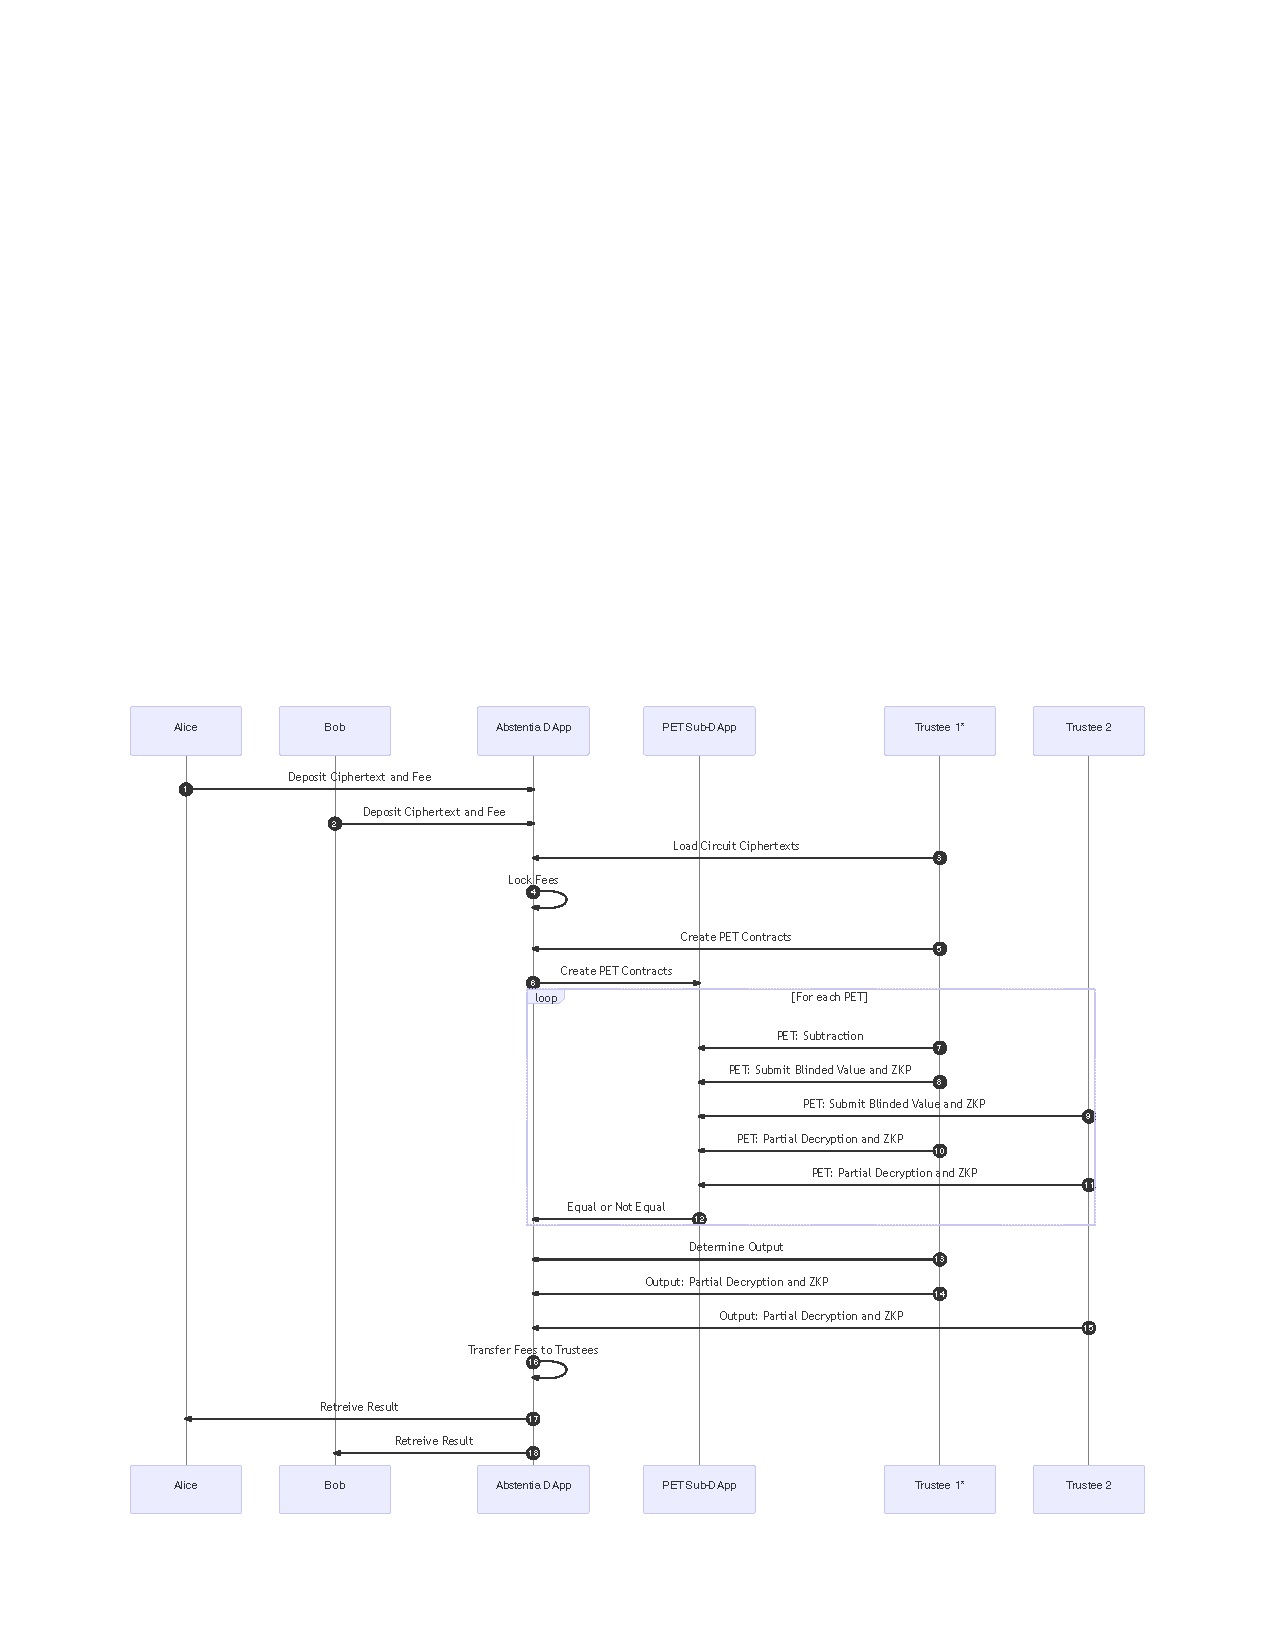
\includegraphics[width=1\textwidth]{figures/absentia.pdf}
	\caption{System overview}
	\centering
	\label{fig:system}
\end{figure}

% = = = = = = = = = = = = = = = = = = = = = = = = = = = = = 

\paragraph{High level flow.} 
%Figure 1. Participants. What they do. Emphasize it just verification and not actual computation. Relate it to Mix and Match as explained above. 
Figure~\ref{fig:system} illustrates the high level overview of the system and how the participants interact with the DApps. The system is composed of a smart contract, called Absentia-DApp (mixmatch.sol), and a sub-module called PET Sub-DApp (PET.sol). Mix and Match is done offline and the Ethereum blockchain is used to perform the verifications that the trustees performed the steps of Mix and Match correctly. Trustees post the proofs related to randomization and partial decryption on chain.

At the beginning of the protocol, Alice and Bob deposit enough funds which will be transferred to the trustees when the protocol ends. They can deposit money any time they want during the protocol. They also load their ciphertexts. Apart from these functions they perform, they do not have to perform any other function during the execution of the protocol. 
 
Trustee 1 is designated as the manager. As Absentia is a submit-and-go  protocol, we prefer to designate a trustee to be the manager and run the functions that can otherwise be run by any other participant. Alternatively, we can have a third party that perform these computations. 

Trustee 1 is responsible for creating the PET contracts and loading the output values for each row at the beginning of the protocol. For each PET, Trustee 1 performs the subtraction. Again for each PET, both Trustee 1 and Trustee 2 proves in zero knowledge that the randomization of the subtraction result is correct and the partial decryption is done correctly. Trustee 1 fully decrypts the result of the subtraction at the end of each PET. During the online phase of Mix and Match, after 8 PETs are performed, Trustee 1 finds the matching row and the corresponding encrypted value. Trustee 1 and Trustee 2 partially decrypt and prove in zero knowledge again to obtain the decrypted result.

% = = = = = = = = = = = = = = = = = = = = = = = = = = = = = 

\paragraph{Payments.}
% What we do for now. Pointer to discussion section for other options. 

Alice and Bob should deposit enough funds before the protocol starts. Alice and Bob can withdraw all the funds they deposited before the protocol starts, at the end of the protocol or after a certain amount of time passes. They can also transfer themselves the extra funds they have deposited, any time during the execution of the protocol, as long as there are enough funds left to pay the trustees. Funds are transferred to the trustees at the end of the protocol, after they determine the final output. The payment schemes are designed to be resistant to reentrancy attacks by using the a modifier that prevent reentrant calls~\footnote{\url{https://github.com/OpenZeppelin/openzeppelin-contracts/blob/master/contracts/utils/ReentrancyGuard.sol}}.

Other possible design choices for the payment scheme:

Trustees can be paid after each task they finish, rather than being paid at the end of the protocol.

The amount of payment can be made proportional to the work they perform.

%In another possible design, trustees can be paid at each step they performed towards reaching the final output.

%  is used to prevent reentrancy attack.

% = = = = = = = = = = = = = = = = = = = = = = = = = = = = = 

\paragraph{Code layout.} 
%Details of testing platform (solidity, \etc). Link to Github. Mathematica is doing what? Solidity is doing what? On Ethereum: Library (why?). PET as module. Factory design (why?) 

Absentia is implemented in Mathematica to have test vectors for the smart contracts written in Solidity and verification for offline computations are performed by the smart contracts using these test vectors~\footnote{Github: link removed for anonymity}. Mixmatch.sol and PET.sol  consists of 214 and 388 lines (SLOC) of Solidity code respectively. ec. sol is the library we use for elliptic curve operations, in order to decrease the gas usage and enhance reusability~\footnote{\url{https://github.com/orbs-network/elliptic-curve-solidity/blob/master/ECops.sol}}. 

As multiplication is an expensive function, we do not perform the multiplication itself in the smart contract. Instead, we use a function called~\emph{ecmulVerify}  ~\footnote{\url{https://ethresear.ch/t/you-can-kinda-abuse-ecrecover-to-do-ecmul-in-secp256k1-today/2384}}. Multiplication is performed off-chain. The function ~\emph{ecmulVerify}  takes the multiplicand, scalar and the product as input and verifies that the multiplication is done correctly. As we perform the computations needed for Mix and Match protocol offline and perform only the verification on chain, we can use this kind of trick to avoid performing multiplications on chain.

Factory design pattern is used in the system. Mix and match contract creates instances of PET contract for each cell in the lookup table, so that Alice and Bob's inputs are compared against related cells. Both contracts follow the order of the functions through state changes. When all PETs are performed, mixmatch contract obtains the final output by finding the matching row.

The measurements show that factory pattern is expensive to realize: create row function in mix and match contract creates two instances of PET contract and it costs $8,741,453$ gas, which is the most expensive function in the system, as the bytecode for PET should be duplicated to create different instances of the contract each time mixmatch runs create row function(see Table~\ref{tab:gascost}). 

In out current design, Alice and Bob have to deposit their inputs again for each PET contract created (8 in total). In another design pattern, we can let Alice and Bob deposit their inputs once to the main contract and then the inputs are loaded to the instances of PET by the main contract. 

% = = = = = = = = = = = = = = = = = = = = = = = = = = = = = 

\subsection{Measurements}

% = = = = = = = = = = = = = = = = = = = = = = = = = = = = = 

\paragraph{Testing platform.} 
%Truffle. Private network. Custom settings (forward pointer for reason to below). 
The smart contracts in Absentia are deployed and tested using Truffle on a local blockchain. We used a custom setting for the gas limit and the contract size. We will explain the reasons to do so below.

~\textcolor{red}{TO-DO:} comparing, testing the results between Mathematica and Truffle.

% = = = = = = = = = = = = = = = = = = = = = = = = = = = = = 

% !TEX root = ../main.tex

\begin{table}[t]
	\centering
	\begin{tabular}{|l|r|}
		\hline
		~\textbf{Code}	& ~\textbf{Size(bytes)}  \\ \hline
		bytecode	& 27178  \\ \hline
		deployed	& 26774  \\ \hline
		initialisation and constructor code 	& 404 \\ \hline
	\end{tabular}
	\caption{Code size for mixmatch.sol}
	\label{tab:codesize}
\end{table}

\paragraph{Code size.} 
%Various sizes. Limits of Ethereum. Consequences (changing limit in truffle). Explain table.

The code size for the mixmatch contract is outlined in Table~\ref{tab:codesize}.  When the contract is deployed, the constructor is run once. The size of the constructor is recorded as 404 bytes. The total size of the bytecode is $27,178$ bytes. Contract size limit is 24KB according to EIP170. As our main contract's size for the deployed code ($26,774$) is over this limit, we ran our test in Truffle by allowing unlimited contract size. We can decrease the contract size by minimizing the code. One solution can be not following the factory design and instead, designating Trustee1 to create 8 PET contracts.


% = = = = = = = = = = = = = = = = = = = = = = = = = = = = = 

% !TEX root = ../main.tex

%~\textbf{Alice:} can call loadFunds more than once. loadCiphertexts  x 4

%~\textbf{Bob:} can call loadFunds more than once. loadCiphertexts x 4

%~\textbf{Trustee1:} is also the manager. Trustee1 calls  
%\begin{enumerate}
%	\item loadOutputs  x 2
%	\item  createRow1  x 4
%\end{enumerate}
%at the beginning of the protocol. 
%\newline
%
%The following is repeated for each PET (8 times): 
%\begin{enumerate}
%	\item PET\_subtract
%	\item DHProve\_Trustee1Pf\_Rand
%	\item DHProve\_Trustee1Pf\_PartialDec
%	 \item FullDecryption
%\end{enumerate}
%
%After all PETs are run, Trustee1 has to run the following:
%\begin{enumerate}
%	\item matchingRow
%	\item matchingValue
%	\item createFinalDecryption
%	\item loadFinalCiphertext
%	\item DHProve\_Trustee1Pf\_PartialDec
%	\item FullDecryption
%\end{enumerate}
%
%~\textbf{Trustee2:} 
%
%The following is repeated for each PET (8 times): 
%\begin{enumerate}
%	\item DHProve\_Trustee2Pf\_Rand 
%	\item DHProve\_Trustee2Pf\_PartialDec
%\end{enumerate}
%and calls DHProve\_Trustee2Pf\_PartialDec once for the final decryption.


\begin{table}[t]
		\centering
	\begin{tabular}{|l|l|r|r|}
		\hline
		~\textbf{Contract} & ~\textbf{Function } & ~\textbf{Gas}  & ~\textbf{Gas Cost (\$)}  \\ \hline
			ec.sol	& Deploy Contract &595,517 & 31.94 \\ \hline

		\multirow{8}{*}{}  
		& Deploy Contract &6,091,398 & 326.75 \\ \cline{2-4} 
		& A\&B: Load Funds & 28,040  &1.50  \\ \cline{2-4} 
	%	& Check Balances &  30,359& 1.63 \\  \cline{2-4} 
		& T1*: Load Outputs&  300,798 & 16.13 \\  \cline{2-4} 
		& T1*: Create Row & 8,741,453 & 468.90 \\  \cline{2-4}
		Mixmatch.sol 	& T1*: Find Matching Row & 37,547 &2.01  \\  \cline{2-4}
		(Absentia DApp)& T1*: Find Matching Value &  40,868&2.19 \\  \cline{2-4}
		& T1*:  Create Final Decryption&  4,430,611& 237.66 \\  \cline{2-4}
		& A\&B: Withdraw Excess Funds &  41,110& 2.21 \\  \cline{2-4}
		&  A\&B:  Withdraw Funds&  39,221& 2.10 \\   \hline
		\multirow{8}{*}{} 
		& Deploy Contract & 4,681,858&251.14 \\ \cline{2-4} 
		&   A\&B or T1*: Load Ciphertexts & 304,668 & 16.34 \\  \cline{2-4}
		& T1*: Subtraction & 242,131 & 12.99\\  \cline{2-4}
		& T1*: Randomization ZKP& 815,340 &  43.74\\  \cline{2-4}
		PET.sol	&  T2: Randomization ZKP& 393,561 &21.11  \\  \cline{2-4}
		(PET Sub-DApp) & T1*: Partial Dec ZKP& 364,298 & 19.54\\  \cline{2-4}
		& T2: Partial Dec ZKP & 363,612 & 19.50 \\  \cline{2-4}
		& T1*: Full Decryption  &  107,086& 5.74 \\  \cline{2-4}
		& T1*:  Load Final Ciphertexts& 173,945 & 9.33\\ \hline
		\cline{1-4}
	\end{tabular}
	\caption{Gas costs per function and who runs the function: Alice (A), Bob (B), Trustee 1 as the leader (T1*), or Trustee 2 (T2). Note that many functions are run more than once.}
	%0.0000536405320861138 USD
	 \label{tab:gascost}
\end{table} 

% !TEX root = ../main.tex

\begin{table}[t]
		\centering
	\begin{tabular}{|l|r|r|r|r|}
		\hline
		& ~\textbf{Alice} &  ~\textbf{Bob} & ~\textbf{Trustee1*}  & ~\textbf{Trustee2}  \\ \hline
		Number of Transactions	& 5 &5  &44  &17  \\ \hline
		Total gas cost	& 1,246,712 &  1,246,712& 52,952,603  & 6,420,996 \\ \hline
		Total cost in USD	&  66.87& 66.87 &2840.41  & 344.43 \\ \hline
	\end{tabular}
	\caption{Cost for each party} 
	\label{tab:participantcost}
\end{table}

% !TEX root = ../main.tex

\begin{table}[t]
		\centering
	\begin{tabular}{|l|r|}
	\hline
	~\textbf{Setting}	& ~\textbf{Total gas}  \\ \hline
	1 gate, 2 trustees	& 61,867,023  \\ \hline
	2 gate, 2 trustees	&  121,240,622 \\ \hline
	1 gate, 3 trustees	& 68,288,019 \\ \hline
\end{tabular}
	\caption{Different settings}
	\label{tab:settings}
\end{table}

\paragraph{Gas costs.} 

%Explain Tables (per function, per participant). Clarify what exactly T1 does. Details of gas to USD.

Table~\ref{tab:gascost} illustrates the cost of deployment of all contracts needed in Absentia and the functions in the two main contracts. The gas costs are recorded using local blockhain provided by Truffle. To calculate the gas costs, we used 1 gas = 87 Gwei as recorded on Dec 01, 2020~\footnote{https://etherscan.io/chart/gasprice}. The price of ETH is $\$615.07$ for the same date~\footnote{\url{https://coinmarketcap.com/currencies/ethereum/historical-data/}}. %The function Create Row creates two instances of PET contract and it is the most expensive function compared to other functions. 

Trustee 1 has to perform more operations than the other participants as the manager (see Table~\ref{tab:participantcost}). In addition to proofs Trustee 1 has to perform for randomization and partial decryption, Trustee 1 also loads the output values of the lookup table into the contract and determines the final output at the end of the protocol.

The total transaction count for each participant can be decreased by using other design choices. As this is a proof-of-concept code, we aimed to logically separate the functions even though they perform the exact same operation. For instance, ZKP for randomization for Trustee1 and Trustee 2 are two separate functions, even though they essentially perform the same ZKP. Separating the logic like this helped us to better differentiate the computations that should be done by each participant. Another way to decrease the number of transactions is to combine operations in a single function. Trustee 1 can perform subtraction, ZKP for randomization and ZKP for partial decryption in a single function.

Even though Trustee 1 and Trustee 2 randomization ZKP functions are the same, there is a difference in the gas costs. $815,340$ and $393,561$ for Trustee 1 and Trustee 2 respectively. The reason is that, when Trustee 1's function is run first, new storage is created to hold the necessary values for the ZKP. But, Trustee 2 overwrites these values, which is a cheaper operation.

Table~\ref{tab:settings} compares how the gas costs differ at different settings compared to our main setting, where two trustees evaluate one gate. When we want to evaluate two circuits, Alice and Bob still perform the same number of transactions, as for the setting where the output of a gate is fed into the other gate, they have to submit their ciphertexts once. We can assume that Trustee 1 loads the inputs for the second gate. The work for Trustee 1 and Trustee 2 is doubled, as they have to evaluate two gates. The cost for the setting, where 3 Trustees are used to evaluate one gate is closer to the cost of the main setting, as the extra cost from Trustee 3 will be the same as Trustee 2.


% = = = = = = = = = = = = = = = = = = = = = = = = = = = = = 
% = = = Arbitrum 
% = = = = = = = = = = = = = = = = = = = = = = = = = = = = = 

\section{Absentia on Layer 2 }
\label{sec:arb}

\subsection{Roll-ups}

A loose collection of technologies, called \emph{Layer 2} solutions, have been proposed to address certain shortcomings of operating directly on Ethereum (\emph{Layer 1}) or other blockchains~\cite{GMR+20}. These solutions generally strive for one or more of the following: reducing transaction latency, increasing transaction throughput, or reducing gas costs. In the case of Absentia, reducing gas costs is paramount. However Layer 2 solutions can also change the threat model; for Absentia, we require that Alice and Bob can trust the final output without having to verify any proofs themselves. 

The most appropriate layer 2 technology for our requirements is called a \emph{roll-up} which targets gas costs. In Ethereum, every transaction is executed (and thus validated) by every Ethereum node. In a roll-up, transactions are executed by off-chain nodes called \emph{validators}. Validators try to convince the Ethereum network that the result of the transaction execution (\ie the state change of the EVM) is correct without the Ethereum nodes having to execute it. 

Since Ethereum nodes cannot just ignore the Ethereum protocol's specifications for how to validate transactions, the roll-up cannot be implemented on Layer 1. Rather it is implemented inside its own DApp (Layer 2). This Layer 2 DApp is effectively a container, operating by its own custom consensus rules, for DApps that want roll-up functionality. The tradeoff is they are isolated from regular L1 DApps without some additional protocols (\eg interoperability support for currency/token transfers and external function calls). For Absentia, we do not require interoperability with L1 other than having a currency in L2 to pay the trustees.

There are at least two ways to convince on-chain participants that an off-chain computation was performed correctly. The first is to prove it with a succinct proof. SNARKS are one proof-type for general computations that are more efficient to verify than performing the computation itself. A second approach (called an \emph{optimistic rollup}) is to have a validator assert the result and then allow for anyone to dispute it before finalizing it. Resolving disputes is always possible by having the Ethereum nodes perform the computation itself, but disputes can be settled in a more succinct way (see \cite{KGCWF18}). If Alice demonstrates that a validator is wrong, the validator is financially punished and Alice is rewarded. Such validators do less work than Ethereum nodes (as well as validators that have to produce SNARKs)---therefore, optimistic rollups enable substantially lower gas costs.

\subsection{Arbitrum}

\begin{figure}[t]
	\centering
	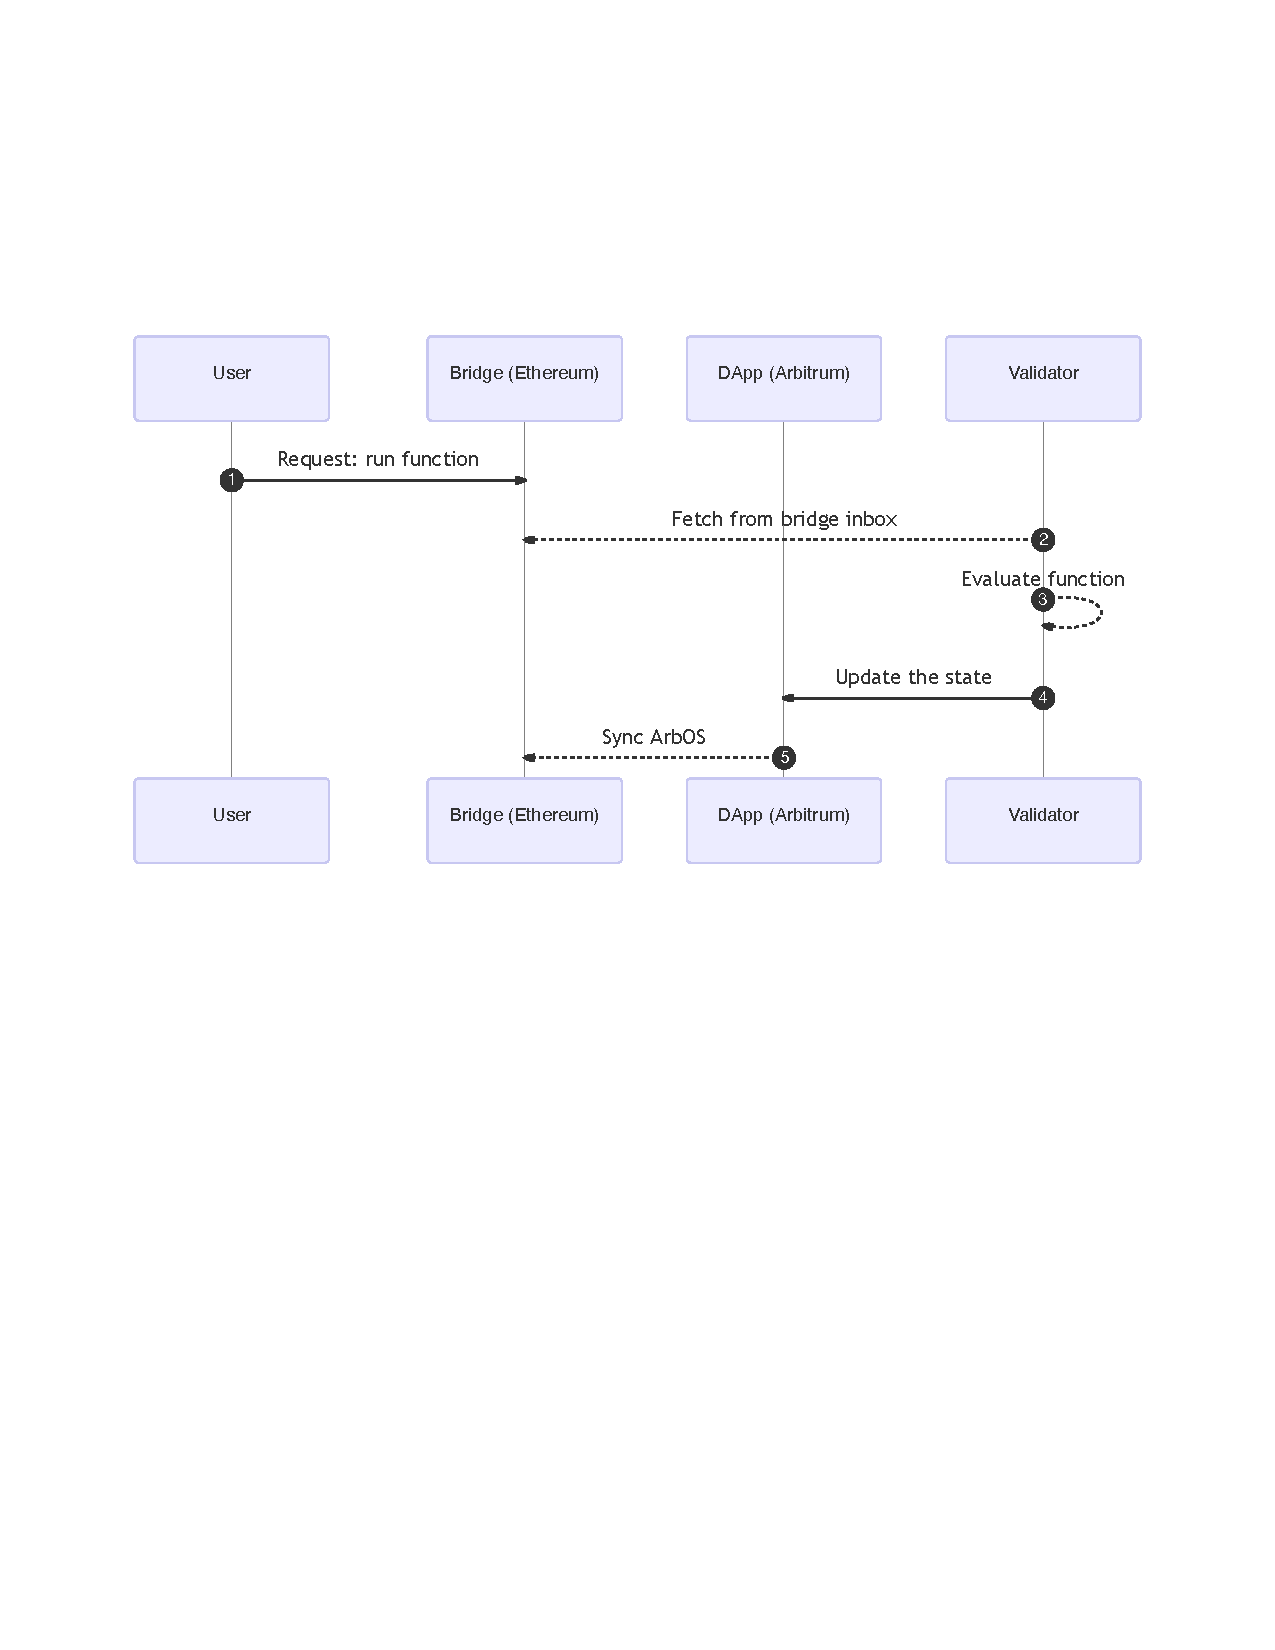
\includegraphics[width=0.8\textwidth]{figures/arbitrum.pdf}
	\caption{Overview of Arbitrum transaction submission.}
	\label{fig:arbsys}
\end{figure}

Arbitrum is Layer 2 solution proposed in a \textit{USENIX Security} paper~\cite{KGCWF18} and now maintained as a commercial project by Offchain Labs. Currently, they operate an optimistic rollup on Ethereum. Instead of operating all Arbitrum contracts (called \emph{ArbOS}) in a container DApp on Ethereum, ArbOS instead operates as a side-chain. A  \emph{bridge contract} on Ethereum serves as an interface between Ethereum and Arbitrum. Figure~\ref{fig:arbsys} shows how function calls work on Arbitrum. A user initiates a transaction on Ethereum to the Bridge Contract with the instruction to deploy a contract or run a function, along with all the data required for Arbitrum to perform this transaction. A validator sees new transactions in the inbox of the bridge, executes one and asserts the result to ArbOS. After a dispute period, the transaction is consider finalized. Periodically, the entire state of ArbOS is committed back to Ethereum. As all Arbitrum transactions are recorded on Ethereum, anyone can compute and compare the current ArbOS state.  

\subsection{Absentia on Arbitrum}

\paragraph{Testing platform.} Arbitrum runs a testnet with a bridge on Ethereum's Kovan testnet. As mentioned above, Absentia is too large to deploy (as a factory contract) within Ethereum's contract size limit. To experiment with Arbitrum, we implement only the PET sub-module as a standalone contract. We run the tests with Truffle. Instead of sending transactions to the Arbitrum bridge (as in Figure~\ref{fig:arbsys}), Arbitrum allows transactions to be sent to relay server (called an \emph{Aggregator}) which will batch all pending transactions together as a single Kovan transaction to the bridge (and pay the gas). However we report the measurements as if the participants were sending the transactions themselves.

% !TEX root = ../main.tex

\begin{table}[t]
	\centering
	\begin{tabular}{|l|r|r|r|r|r|r|r|}
		\hline
		&    \multicolumn{2}{c|}{~\textbf{Ethereum}} & \multicolumn{5}{c|}{~\textbf{Arbitrum}} \\ \hline
		~\textbf{Function}  &  &    & ~\textbf{ L1} & ~\textbf{L1}  & ~\textbf{L2} &~\textbf{L2}&  \\ 
		&~\textbf{Tx} &~\textbf{Gas}  &~\textbf{Tx} &  ~\textbf{Gas} & ~\textbf{Tx}&~\textbf{ArbGas}&~\textbf{Size}  \\ 
		\hline
		Deploy ec &  ~\href{https://kovan.etherscan.io/tx/0x088af056a640c1fe2188678e52484f89b7ba0bd9345bb0578d91c96aa480c59c}{Link}& 1,103,372& ~\href{https://kovan.etherscan.io/tx/0xa80f0eb0408f8f1c760abbc223b6a3b24780aba4b85f96ecbd6fb0dfe94bd606}{Link}&80,152& ~\href{https://explorer.offchainlabs.com/#/tx/0x7c82717b52cb133c8855c0833d3cbf9ded19f884764fce78de3bb4e27feb63cd}{Link}&1,304,481&4978\\  \cline{1-8}
		
		Deploy PET &  ~\href{https://kovan.etherscan.io/tx/0xb76cda2c91907234afc0b971df893a6dbcdf83d482d2ff3d7d29b4a0b313002f}{Link}&5,266,352& ~\href{https://kovan.etherscan.io/tx/0x2ec73b92474c991d7b9f8ad1c46f95ef9125513897badb0c0c5faa19bd5b9a55}{Link}&386,079& ~\href{https://explorer.offchainlabs.com/#/tx/0x2b1e63c81ca8ab7f4a6fe5333daab515a4e7408121771ae58e205ee037bceb50}{Link}&4,260,273&24,172\\  \cline{1-8}
		
		Load Ciphertexts  & ~\href{https://kovan.etherscan.io/tx/0x2cb4bf0f6ce9fc7cabf0c152fdc61ccfff00a0f2e717c85da7eab806fa101b5b}{Link}&305,309 &  \href{https://kovan.etherscan.io/tx/0x612e19481fff4ddd1c2dfe260908f15c7c74072a1e733597b4bab1c1209169f4}{Link}& 7869 &\href{https://explorer.offchainlabs.com/#/tx/0x28b3fa1a91d6d6e13005d352940861a026ac029fbc13a58dc969e98ffb5b392c}{Link} &  820,507& 742\\  \cline{1-8}
		
		Subtraction & ~\href{https://kovan.etherscan.io/tx/0x6eeb3031c81af252df1fb806ae0a57643c20792df7336004465c6a74792c0016}{Link}&260,729 & ~\href{https://kovan.etherscan.io/tx/0xa31a5653f3bfbdf7bcce4520c2a4f0e8d38fbc5c19036548199f805a4997cf68}{Link} & 5469& ~\href{https://explorer.offchainlabs.com/#/tx/0xbeff60af08f1b88deabe690322e26794d87595b332f1f1d01095a6a4528c4254}{Link} & 4,789,799& 550\\  \cline{1-8}
		
		T1 Randomization ZKP &~\href{https://kovan.etherscan.io/tx/0x30e8ccff5af6f3489ba2dc11e3198f0216487f380aa2a66ddf97e94650490e88}{Link} &819,877 &  ~\href{https://kovan.etherscan.io/tx/0xc08cc82908b7e87e8ddc75695c4f29c3bce3d9a8caced144f003c59e23f4690e}{Link}&  11,488&  ~\href{https://explorer.offchainlabs.com/#/tx/0xe3d1ba8bc653397dd67f3bfb602db0acce617668dc2ae2f30e038b4137a60e24}{Link}& 10,972,720& 644\\  \cline{1-8}
		
		T2 Randomization ZKP & ~\href{https://kovan.etherscan.io/tx/0x6dd05a76c771089144583a685c2fb9a6b566a626aa86b568230faf83268fdd92}{Link}& 398,245 & ~\href{https://kovan.etherscan.io/tx/0xd790b2edd8800a183068b3253d7e5b00e57d850bce8d9b8572494539b58c7e3c}{Link} &11,440& ~\href{https://explorer.offchainlabs.com/#/tx/0x71535a6b6d0124cbd61a4993e5e831cc4ba151eec60b1c368a79686f3f5bc1f4}{Link} & 11,069,485 & 742 \\  \cline{1-8}
		
		T1 Partial Dec ZKP &~\href{https://kovan.etherscan.io/tx/0x477b3e6b645cc672bbbe99ea3e7fa227962a3e1222071c266442a5ab8366e1bb}{Link} &366,636 & ~\href{https://kovan.etherscan.io/tx/0xdd0ffc715dc5733bee36fd99d51898cf978de27ece76777099c4570929039a25}{Link} & 11,452& ~\href{https://explorer.offchainlabs.com/#/tx/0x9f7fba14177790f6dad6ad9bb0ec3017803b466a27182768b11163162a3961c3}{Link} & 10,692,786& 742\\  \cline{1-8}
		
		T2 Partial Dec ZKP &~\href{https://kovan.etherscan.io/tx/0x59a6282197cbd71b2c25cd5f3547b41ca7baf33322088f35273c97fce5cf8b56}{Link} &366,089 & ~\href{https://kovan.etherscan.io/tx/0xb2a71505f192dd2119634ddd69070c52eb3a3d993aeb632ea8f823eb62f26e84}{Link} & 11,512&  ~\href{https://explorer.offchainlabs.com/#/tx/0x724578f12940ebd653613c5037576540ce129ef277e4db67aff135711327e8f8}{Link} & 10,689,113& 742\\  \cline{1-8}
		
		Full Decryption & ~\href{https://kovan.etherscan.io/tx/0x172804db2abcef274dedfad8f31f84a0bb26c87826842589537f1d511402b282}{Link} & 124,816 &  ~\href{https://kovan.etherscan.io/tx/0x10788165eacbbe25066c163fa0cf7a5af07da32c05af001d0f05ad8946974c6e}{Link}& 6236& ~\href{https://explorer.offchainlabs.com/#/tx/0x3515cc045805f2f9af9f378f4725ab4845679ca15ecd2e86758f8d53eb9a7353}{Link} & 4,258,675 & 422\\  \hline
	\end{tabular}
	\caption{Comparison between deploying a plaintext equality test on Ethereum and deploying on Arbitrum (via Ethereum). The links show the reader the actual transactions of a test-run on Kovan/Arbitrum's respective block explorers. Size is the calldata in bytes.} 
	\label{tab:arbgas}
\end{table}

\paragraph{Gas costs.} Table~\ref{tab:arbgas} compares the cost of running a plaintext equality test (PET) on Ethereum (specifically Kovan testnet) and running it on Layer 2 (L2) with Arbitrum. Note the Ethereum numbers differ slightly from Table~\ref{tab:gascost} as it is deployed on a different testnet (Kovan instead of private) and we modified it slightly to be a stand-alone DApp.

Arbitrum creates two transactions (recall Figure~\ref{fig:arbsys}): the Ethereum gas cost of relaying the (layer 1 or L1) transaction to the Arbitrum bridge, and the cost for the validator to execute the function, measured in ArbGas. The cost of the first Arbitrum transaction (\emph{L1 Gas}) is paid with ETH but is invariant to its computational complexity. It is essentially only a function of its size (compare \emph{L1 Gas} to \emph{Size}).  Note that the gas costs listed on the Kovan block explorer (links under \emph{L1 Tx}) are for aggregated batches of transactions. We report what the cost would be to send it directly (not through an aggregator).

The ArbGas cost on Arbitrum should be similar to the gas cost on Ethereum, however validators do not run EVM bytecode directly. It is translated into Arbitrum virtual machine (AVM) bytecode which has its own opcodes and ArbGas costs. ArbGas has no market price currently. It is expected to be much cheaper than Ethereum's gas. In practice, the trustees could act as validators for Absentia transactions as they have to perform the computation anyways. Therefore we approximate arbgas as free.

A run of PET on Ethereum costs 9,011,425 gas (or 483.38 USD), while on Arbitrum the cost is 531,697 gas (or 28.52 USD). In this use case, Arbitrum reduces Ethereum gas costs by 94\%.  




% = = = = = = = = = = = = = = = = = = = = = = = = = = = = = 
% = = = Discussion 
% = = = = = = = = = = = = = = = = = = = = = = = = = = = = = 

\section{Discussion}
\label{sec:discussion}
\begin{itemize}
\item Payments: fancier, contingent on who aborts, timeliness, \etc
\item Pre-comp: validate it , have pre-built and validated circuits, \etc
\item Implementation improvements: factory design and contract size
\item Proxy re-encryption instead of decryption
\item what else?
\end{itemize}

% = = = = = = = = = = = = = = = = = = = = = = = = = = = = = 
% = = = Conclusions
% = = = = = = = = = = = = = = = = = = = = = = = = = = = = = 

\section{Concluding Remarks}
